\documentclass[conference]{IEEEtran}
\IEEEoverridecommandlockouts
% The preceding line is only needed to identify funding in the first footnote. If that is unneeded, please comment it out.
\usepackage{cite}
\usepackage{amsmath,amssymb,amsfonts}
\usepackage{algorithm}
\usepackage{algpseudocode}
\usepackage{graphicx}
\usepackage{textcomp}
\usepackage{xcolor}
\usepackage{subcaption}
\usepackage{animate}

\def\BibTeX{{\rm B\kern-.05em{\sc i\kern-.025em b}\kern-.08em
    T\kern-.1667em\lower.7ex\hbox{E}\kern-.125emX}}
\begin{document}

\title{ECE276B PR3 Report}

\author{
\IEEEauthorblockN{1\textsuperscript{st} Weixiao Zhan}
\IEEEauthorblockA{
    weixiao-zhan[at]ucsd[dot]edu}
}

\maketitle

\section{Introduction}
This project aims to develop a safe trajectory tracking policy 
for a ground differential-drive robot operating 
under a discrete periodic time horizon.
The trajectory tracking problem is formulated as a 
discounted infinite-horizon stochastic optimal control problem.
The control policy must track a desired reference trajectory 
while managing a noisy motion model and avoiding obstacles. 

This project explores two primary approaches: 
receding-horizon certainty equivalent control (CEC) and 
generalized policy iteration (GPI), specifically the Q-value iteration. 
The performance of both methods is evaluated based on 
tracking accuracy, computational complexity, and collision avoidance capabilities.


\section{Problem Formulation}
\subsection{Environment}
The environment in which the robot operates has following characteristics:
The \(xy\)-plane is bounded within \([-3, 3] \times [-3, 3]\).
There are two circular obstacles:
Obstacle \( C_1 \) is centered at \((-2, -2)\) with a radius of 0.5.
Obstacle \( C_2 \) is centered at \((1, 2)\) with a radius of 0.5.
Denote the free space:
\[ \mathcal{F} = [-3, 3]^2 \setminus (C_1 \cup C_2) \]

The reference trajectory is a sequence of positions and orientations:
\[ r_t \in [-3,3] \times [-3,3] \times [-\pi, \pi)\]
Note that reference trajectory may overlap with obstacles.
And the control policy need to avoid the obstacles.

\subsection{Motion Model}
The motion model of the differential-drive robot is defined as follows. 
The robot's state at time \( t \), denoted by 
\( {x}_t = ({p}_t, \theta_t) \), 
consists of its position \( {p}_t \in [-3,3]^2 \) and orientation \( \theta_t \in \mathbb{R} \). 
The control input \( {u}_t = (v_t, \omega_t) \) 
consists of the linear velocity \( v_t \in [0,1] \) and 
angular velocity \( \omega_t \in [-1,1] \). 
The discrete-time kinematic model, 
derived from Euler discretization with a time interval \( \Delta > 0 \), is:

\[
{x}_{t+1} = {f}({x}_t, {u}_t, {w}_t) = {x}_t + {G}({x}_t) {u}_t + {w}_t
\]
where
\[
{G}({x}_t) = \begin{bmatrix}
\Delta \cos(\theta_t) & 0 \\
\Delta \sin(\theta_t) & 0 \\
0 & \Delta 
\end{bmatrix}
\]
and motion noise \( {w}_t \sim \mathcal{N}(0, \Sigma) \).

\subsection{Receding-horizon CEC}
CEC is a suboptimal open-loop-feedback control scheme.
It, at each stage, applies the control that would be optimal,
if the noise variable $w_t$ were realized at their expected values. 
The main advantage of CEC is that it reduces 
a stochastic optimal control problem to a deterministic optimal control problem, 
which can be solved more effectively. 

In addition,
receding-horizon CEC approximates infinite-horizon problem 
by repeatedly solving the following discounted finite-horizon
deterministic optimal control problem at each time step.

Formally, when given state $x_\tau$, 
CEC solves following optimization problem to find control sequence $u_{\tau:\tau+T-1}$, 
applies the first control $u_\tau$, then uses the realization of $x_{\tau+1}$ for next stage.
\[
\begin{gathered}
\min_{{u}_\tau, \ldots, {u}_{\tau+T-1}} 
q({e}_{\tau+T}) + 
\sum_{t=\tau}^{\tau+T-1} \gamma^{t-\tau} 
\left( 
    \begin{gathered}
        \tilde{p}_t^\top Q \tilde{p}_t  \\ 
        +\\
        q(1 - \cos(\tilde{\theta}_t))^2 \\
        +\\
        {u}_t^\top R {u}_t 
    \end{gathered} 
\right) \\
s.t. \left\{
\begin{aligned}
{e}_{t} 
    &= x_{t} - r_{t} \\
    &= \left[\begin{matrix}\tilde{p}_t&\tilde{\theta}_t\end{matrix}\right]^T \\
x_{t} 
    &= f({x}_{t-1}, {u}_{t-1}, 0) \\
    &= \left[ \begin{matrix}p_{t} & \theta_{t} \end{matrix}  \right]^T \\
{p}_t
    &\in \mathcal{F} \\
{u}_t
    &\in \mathcal{U} \\
\end{aligned}
\middle|
\begin{aligned}
    x_\tau\\
    T &\in \mathbb{N}^+\\
    Q &\in \mathbb{R}^{[2\times 2]} \\
    q &\in \mathbb{R} \\
    R &\in \mathbb{R}^{[2\times 2]}
\end{aligned}
\right.
\end{gathered}
\]
in which, $T$ is the look ahead steps, 
$Q,q,R$ are loss function hyper-parameters.

\subsection{Non-linear Programming (NLP)}
An NLP program written in following standard form can be solved by an NLP solver.
\[
\begin{aligned}
&\min_{{U}} & & c({U}, {E}) \\
&\text{subject to} & & {U}_{\text{lb}} \leq {U} \leq {U}_{\text{ub}} \\
& & & {h}_{\text{lb}} \leq {h}({U}, {E}) \leq {h}_{\text{ub}}
\end{aligned}
\]
where \( {U} = [{u}_\tau^\top, \ldots, {u}_{\tau+T-1}^\top]^\top \) and \( {E} = [{e}_\tau^\top, \ldots, {e}_{\tau+T}^\top]^\top \).

\subsection{GPI}
GPI is a powerful technique to approach 
infinite horizon planing problem.
The standard GPI repeats following two steps until converged:
\subsubsection{policy evaluation} finds value function $V^{\pi}$ of a given policy $\pi$.
\subsubsection{policy improvements} greedy improve the policy.

To use GPI in this problem, discretization or parametrization of value function 
are necessary for computers to handle contiguous state space.

\subsection{Q-value iteration}
Q-value iteration is an equivalent variation of general policy iteration.
Its routines is shown in Algorithm \ref{algo:gpi}.
\begin{algorithm}
    \caption{Q-value iteration}
    \label{algo:gpi}
    \begin{algorithmic}[1] % The number [1] enables line numbering
    \While{$\delta Q > \epsilon$}
        \Comment Q-value iteration
        \State for $\forall x \in \mathcal{X}, u \in \mathcal{U}$
        \State $Q(x,u) = l(x,u) + \gamma \mathbb{E}_{x'\sim p_f}\left[\min_{\forall u' \in \mathcal{U}} Q(x', u')\right]$
        % Your loop code here
    \EndWhile
    \State $\pi(x) \leftarrow \arg\min_u Q(x, u), \forall x$
    \Comment extract policy
    \end{algorithmic}
\end{algorithm}


\section{Technical Approach}

\subsection{Receding-horizon CEC: NLP Formulation}
In this project, the receding-horizon CEC problem is converted into standard NLP form and solved using Casadi library.

\subsubsection{optimization variable}
\[
\begin{aligned}
U&=\left[ \begin{matrix}u_{\tau }&...&u_{\tau +T-1}\end{matrix}  \right] &\in R^{[2\times T]}\\ 
U_{lb}&=\left[ \begin{matrix}0&\cdots &0\\ -1&\cdots &-1\end{matrix}  \right] \\ 
U_{ub}&=\left[ \begin{matrix}1&\cdots &1\\ 1&\cdots &1\end{matrix}  \right] 
\end{aligned} 
\]

\subsubsection{objective}
\[
\begin{gathered}
\begin{aligned}
C(U, x_\tau)
    &=\sum^{\tau +T-1}_{t=\tau } \gamma^{t-\tau } \cdot \left(loss_{e}\left( x_{t}-r_{t} \right) +loss_{u}\left( u_{t} \right)  \right) \\
\end{aligned}
\\ 
\text{in which} \left\{\begin{aligned}
loss_{e}(e_{t})
    &=\underbrace{\tilde{p}^{T}_{t}Q\tilde{p}_{t}}_{A} 
    +\underbrace{q\left( 1-\cos \left( \tilde{\theta}_{t}  \right)  \right)^{2} }_{B} \\ 
loss_{u}(u_{t})
    &=\underbrace{u^{T}_{t}Ru_{t}}_{C} 
    +\underbrace{\left( u_{t}-u_{t-1} \right)^{T} r\left( u_{t}-u_{t-1} \right) }_{D} \\
x_{t}&=f(x_{t-1},u_{t})\\ 
e_{t}&=\left[ \begin{gathered}\tilde{p}_{t}\\ \tilde{\theta}_{t} \end{gathered}  \right]
\end{aligned} \right.
\end{gathered}
\]

The above Formulation hardcoded the motion model $f$, reference trajectory $r_t$,
and error state $e_t$'s calculation into the objective function. 

Term $A$ and $B$ regulates the position and orientation error 
between states and reference trajectory.
Term $C$ regulates large controls.

Term $D$ is an added smoothing term in practice.
Because of the discounted formulation, NLP solver may
delaying controls into future as the quadric term $C$ is exponentially decayed in time,
leads to small controls at $\tau$ state.
Meanwhile, only $u_\tau$ is actually used and $u_{\tau+1:}$ are discarded.
Term $D$ is added to avoid such behavior. 
Its impact is further discussed in Results section.

\subsubsection{constrains}
\[
\begin{gathered}
\begin{aligned}
h(U, x_\tau)&=\left[ \begin{matrix}p_{\tau +1}&\cdots &p_{\tau +T-1}\\ \| p_{t}-c_{1}\|_{2} &\cdots &\| p_{\tau +T-1}-c_{1}\|_{2} \\ \| p_{t}-c_{2}\|_{2} &\cdots &\| p_{\tau +T-1}-c_{2}\|_2 \end{matrix}  \right] \\ 
h_{lb}&=\left[ \begin{matrix}\left[ \begin{gathered}-3\\ -3 \end{gathered}  \right] &\cdots &\left[ \begin{gathered}-3\\ -3 \end{gathered}  \right] \\ c_{1}.r&\cdots &c_{1}.r\\ c_{2}.r&\cdots &c_{2}.r\end{matrix}  \right] \\ 
h_{ub}&=\left[ \begin{matrix}\left[ \begin{gathered} 3\\  3 \end{gathered}  \right] &\cdots &\left[ \begin{gathered} 3\\  3 \end{gathered}  \right] \\ \infty&\cdots &\infty\\ \infty&\cdots &\infty\end{matrix}  \right] 
\end{aligned} \\
\end{gathered} 
\]
in which, 
\( x_{t} = \left[ \begin{gathered}p_{t}\\ \theta_{t} \end{gathered}  \right]  
=f(x_{t-1},u_{t-1}) \)

Similar to objective function, the motion model $f$ is hardcoded into the constrain function.
The constrains enforces the states $x_t$ to be within the free space $\mathcal{F}$.

Since the objective function takes periodic $\cos$ over $\tilde{\theta}$,
the orientation of state \textbf{does not} need to 
normalize into the reference trajectory's orientation space $[-\pi, \pi)$.

\subsubsection{formation considerations}
Converting CEC into the above NLP without explicitly introducing 
optimization variable on state $x_t$ or error states $e_t$ has several benefits.
\begin{itemize}
    \item avoids motion model constrains in following form: 
    \[-\epsilon < x_{t+1} - f(x_t, u_t) <\epsilon\]
    The motion model is now part of the objective and constrain functions.
    \item avoids implementing error state motion model,
    \item avoids boundary and collision check on error states $e_t$ 
    \end{itemize}

The formulation also skipped the stage cost term.
For a conventional stage cost $q(x_{\tau+T}) = \gamma^T (loss_e(e_{\tau+T}) + loss_u(u_{\tau+T}))$,
it would have the same effect of increasing look ahead step by 1, thus skipped.

\subsubsection{hyper-parameter tuning}
In practice, following hyper-parameters produced best results:
\[
\begin{array}{ll}
    T=5
    &\gamma = 0.9\\ 
    Q=\left[ \begin{matrix}2&0\\ 0&2\end{matrix}  \right] 
    &q=2\\ 
    R=\left[ \begin{matrix}0.05&0\\ 0&0.05\end{matrix}  \right] 
    &r=\left[ \begin{matrix}0.05&0\\ 0&0.05\end{matrix}  \right] 
\end{array} 
\]
Different hyper-parameters and their effect are further discussed in Results section.

\subsection{GPI: GPU Batch Q-value iteration}
The computation of Q-value iteration is highly parallelizable, 
making GPUs the ideal hardware to leverage. 
In this project, 
a GPU-accelerated batch Q-value iteration is implemented with PyTorch.

\subsubsection{state space discretization}
The orientation is first normalized into $[-\pi,\pi)$.
The state space $\mathcal{X} = [-3,3]^2\times[-\pi,\pi)$ is
discretized into $(nx, ny, nth)$ equally-spaced points in each dimension.
The control space $\mathcal{U} = [0,1]\times[-1,1]$ is discretized into $(nv,nw)$
equally-spaced controls values.
Since the trajectory has period $\mathcal{T}$, 
the time horizon is discretized in $nt=\mathcal{T}$ steps.

\subsubsection{f:transition matrix and probability}
The continuous and stochastic motion model
\[p_f(\cdot | x, u, w) \]
is discretized and approximated using the following method:

\begin{itemize}
    \item For all discrete state \( x \) and control \( u \),
    a neighborhood with $K$ states, denote as \( \{x'_{k} |k < K\}\), 
    around the mean \(x' = f(x, u, 0) \) in the discretized space 
    is considered possible next states.
    \item  The likelihood of transitioning to \( x'_{0:K-1} \)
    is evaluated using the Gaussian distribution \( N(x', \Sigma) \).
    \item For $x'_k$, that are out of boundary and/or causing collision, 
    their coordinates are clamped and probabilities set to 0.
    \item The transition probability distribution is then normalized within 
    the neighborhood, so that  \(\sum_k p(x'_{k}) = 1\) 
\end{itemize}

The discretization of $f$ can be effectively computed with PyTorch batch and broad cast operations.
The results are saved in two tensors:
transition tensor, $P$ with shape $(K, nx, ny, nth, nv, nw, 3)$, stores the \textbf{indices} of neighborhood points $x'_k$;
transition probabilities tensor, $P_p$ with shape $(K, nx, ny, ,nth, nv, nw)$, stores their probabilities.

Note the transition tensors are discretization of $f$, thus is \textbf{time invariant}.

\subsubsection{stage cost}
$$
\begin{aligned}
l(x_t, u_t) &= 
    \tilde{p}^{T}_{t}Q\tilde{p}_{t} 
    + q\left( 1-\cos \left( \tilde{\theta}_{t}  \right)  \right)^{2} 
    + u^{T}_{t}Ru_{t} \\
s.t. \ \left[ \begin{gathered}\tilde{p}_{t}\\ \tilde{\theta}_{t} \end{gathered}  \right] 
    &= x_{t}-r_{t}
\end{aligned}
$$

The stage cost can be discretized and save to tensor $L$ with shaped $(nt, nx, ny, nth, nv, nw)$.
For those states that are out of boundary and causing collision, 
their stage costs are set to $\infty$

Note the stage cost dependents on the reference trajectory and is \textbf{time variant}.

\subsubsection{Q-value iteration and policy extraction}
implements Algorithm \ref{algo:gpi} using batch operations.
The expectation $E_{x' \sim p_f}$ is approximated by the weighted sum of 
neighbors' V-value at next time step, $t' = (t+1)\mod nt$.
Q values are stored in tensor $Q$, with shape $(nt, nx, ny, nth, nv, nw)$.

Q value iteration is executed until $\|Q_k - Q_{k-1}\| < \delta$.
Then the policy $\pi$ is extract from taking $\arg\min$ over the last two dimensions of $Q$

\subsubsection{implementation considerations}
Similar to CEC approach, 
the standard states and motion model $f$ is discretized instead of the error states.
The primary considerations is memory consumption.
The standard motion model need to discrete $6*6*2\pi*1*2$ hyper-volume 
but the error motion model need to discrete $12*12*2\pi*1*2$ hyper-volume which is 4 times greater.

However, the error state allows adaptive discretization: 
discrete finer near the origin and coarse on the peripheral, 
which is left for future work.

\subsubsection{hyper-parameter tuning}
In practice, GPI used the same $Q,q,R$ as CEC. 
And following discretization perform the best:
\[
\begin{array}{lll}
nt=100&&\\ 
nx=31&ny=31&nth=11\\ 
nv=6&nw=11&\\
K=1&\delta = 10\end{array} 
\]

Because the discretization is relatively sparse compare to the noise variance,
most of the probability weight is concentrated on one or two points in the neighborhood.
A 7-point spindle neighborhood ($K=7$) would consume $7\times$ memory 
compare to $K=1$ neighborhood in batch Q iteration,
which is unfortunately exceeded GPU GRAM capacity.
Thus the nearest point neighborhood ($K=1$) is used.

Those infinite stage costs are set to a large number of $10^{10}$, 
as infinity cause \texttt{nan} in norm computation.

With $\delta=10$, Q-value iteration usually take around 50 iterations.

\section{Results}
Full animated results can be found at \texttt{fig/*.gif}.

Best results of using P-controller CEC, and GPI are present in Figure \ref{fig:best}.
\begin{figure*}
    \centering
    \begin{subfigure}[b]{0.3\textwidth}
        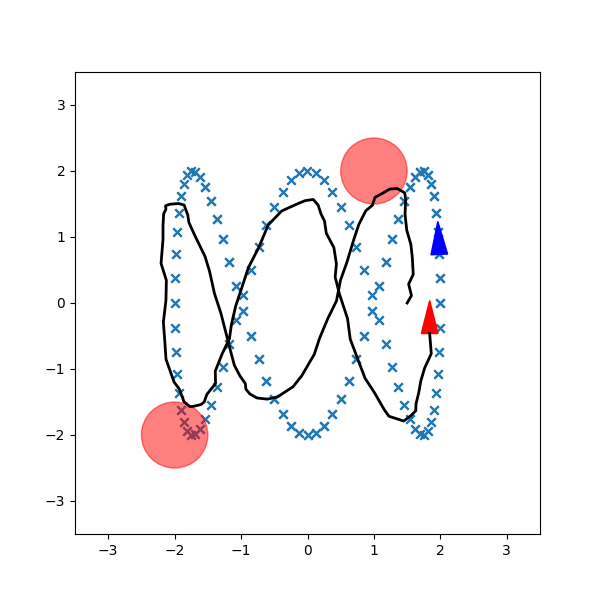
\includegraphics[width=\textwidth]{../fig/p_controller.png}
        \caption{p-controller}
        \label{fig:p-controller}
    \end{subfigure}
    \hfill
    \begin{subfigure}[b]{0.3\textwidth}
        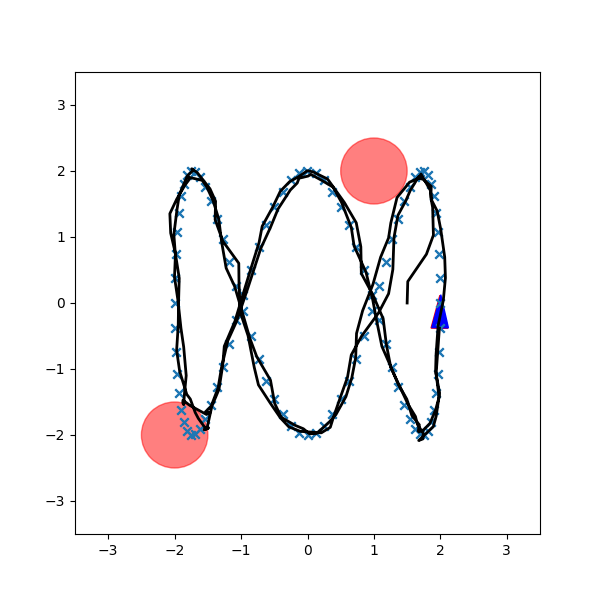
\includegraphics[width=\textwidth]{../fig/trajectory.cec.png}
        \caption{CEC}
        \label{fig:cec}
    \end{subfigure}
    \hfill
    \begin{subfigure}[b]{0.3\textwidth}
        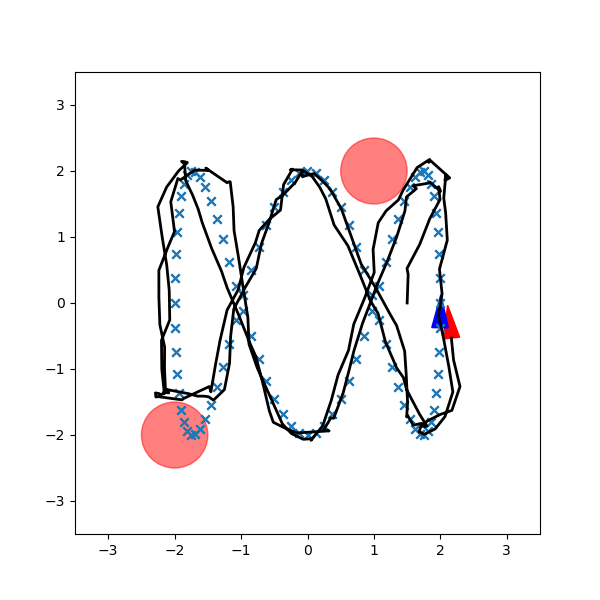
\includegraphics[width=\textwidth]{../fig/trajectory.gpi.png}
        \caption{GPI}
        \label{fig:gpi}
    \end{subfigure}
    \caption{Best results from P-controller, CEC, GPI}
    \label{fig:best}
\end{figure*}

\subsection{CEC}
This section compares results produced by different hyper-parameters of CEC.

\subsubsection{look ahead steps $T$}
Figure \ref{fig:T} shows the effect of changing $T$.
Compare to $T=5$ (Figure \ref{fig:T5})
For a too small $T=1$ (Figure \ref{fig:T1}), the policy won't be able to avoid obstacles in advance.
For a too large $T=20$ (Figure \ref{fig:T1}), the solver converged to a different local optimal, 
it first bypassed the obstacles then chase the trajectory. 
This could due the choose of $\gamma = 0.9$, 
the solver didn't weight the near stages enough.

In addition, larger $T$ would cause CEC much slower to solve. 
$T=25$ is around the limit of finding next control just-in-time on my machine.

\begin{figure*}[h]
    \centering
    \begin{subfigure}[b]{0.3\textwidth}
        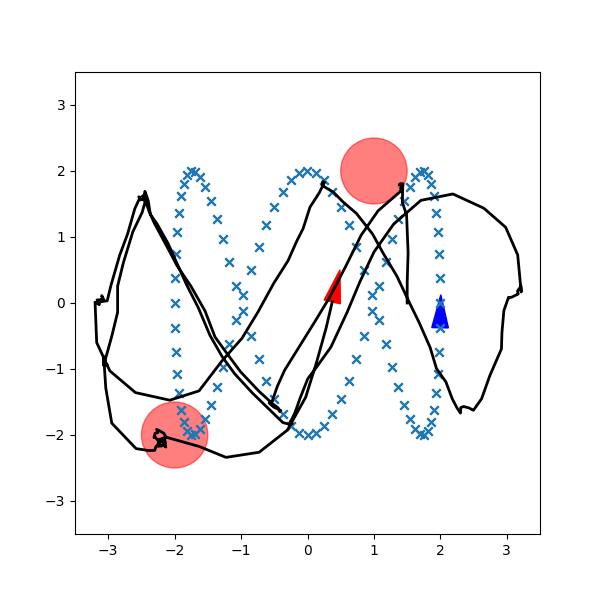
\includegraphics[width=\textwidth]{../fig/trajectory.cec.T_1.png}
        \caption{$T=1$}
        \label{fig:T1}
    \end{subfigure}
    \hfill
    \begin{subfigure}[b]{0.3\textwidth}
        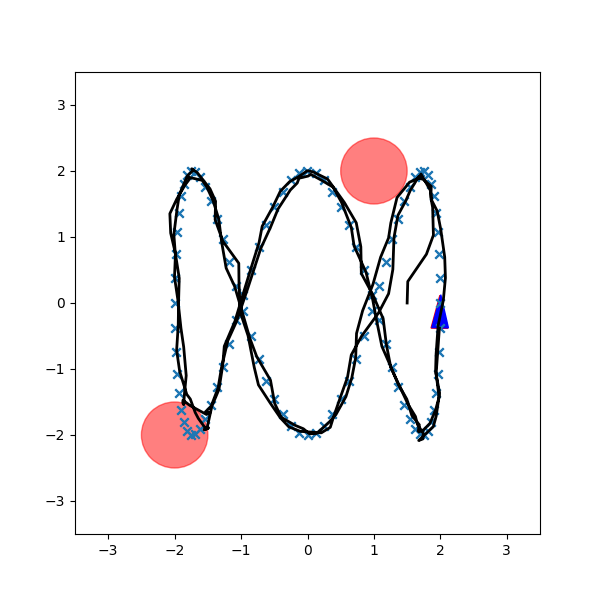
\includegraphics[width=\textwidth]{../fig/trajectory.cec.png}
        \caption{base line $T=5$}
        \label{fig:T5}
    \end{subfigure}
    \hfill
    \begin{subfigure}[b]{0.3\textwidth}
        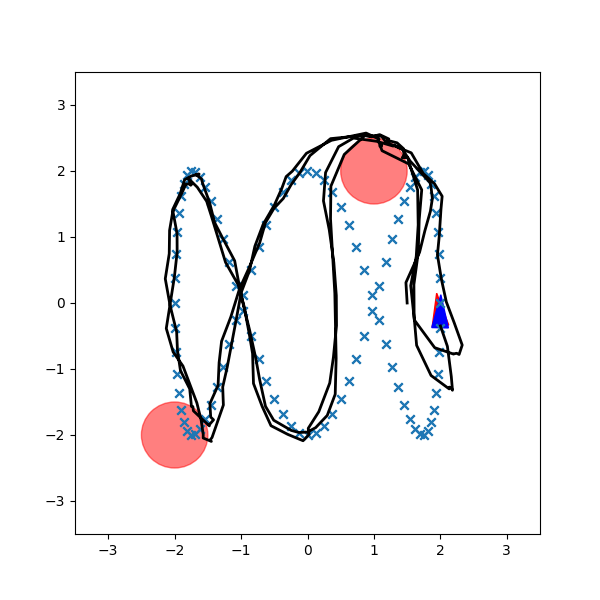
\includegraphics[width=\textwidth]{../fig/trajectory.cec.T_20_0.1.png}
        \caption{$T=20$}
        \label{fig:T20}
    \end{subfigure}
    \caption{look ahead steps}
    \label{fig:T}
\end{figure*}

\subsubsection{smoothing term: $r$}
In the CEC formation, a smoothing term $D$ is added.
Figure \ref{fig:r} shows the result without smoothing and with $r=1$ compare to $r=0.05$ at \ref{fig:r005}.
With the smoothing term, the turns are less sharp, and the trajectory is more smooth.
For a different less smooth reference trajectory, such smoothing term could become useful.

\begin{figure*}[h]
    \centering
    \begin{subfigure}[b]{0.3\textwidth}
        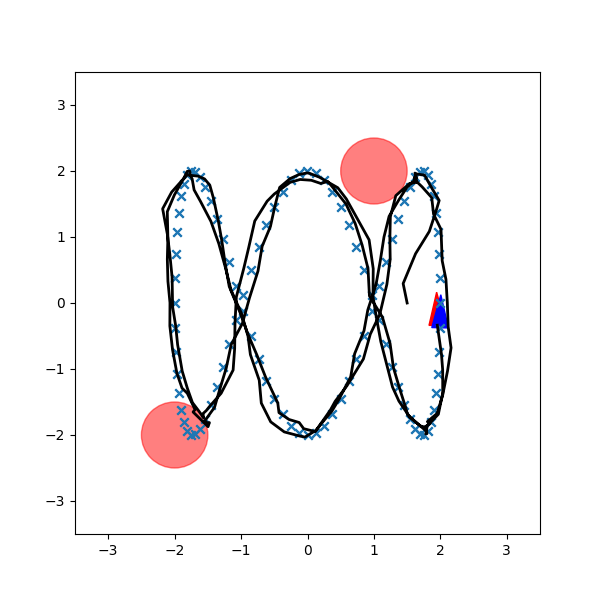
\includegraphics[width=\textwidth]{../fig/trajectory.cec.r_0.png}
        \caption{no smoothing $r=0$}
        \label{fig:r0}
    \end{subfigure}
    \hfill
    \begin{subfigure}[b]{0.3\textwidth}
        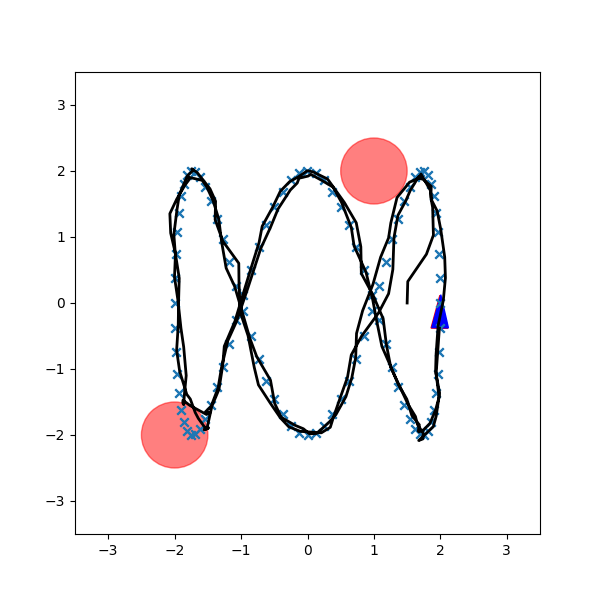
\includegraphics[width=\textwidth]{../fig/trajectory.cec.png}
        \caption{base line $r=0.05$}
        \label{fig:r005}
    \end{subfigure}
    \hfill
    \begin{subfigure}[b]{0.3\textwidth}
        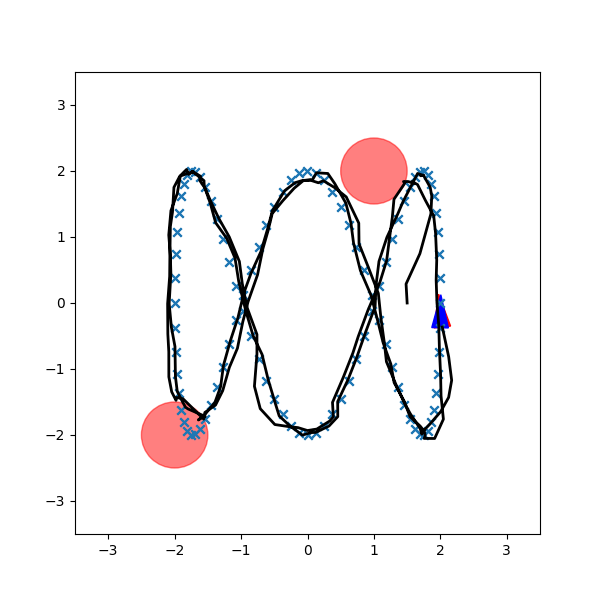
\includegraphics[width=\textwidth]{../fig/trajectory.cec.r_1.png}
        \caption{more smoothing $r=1$}
        \label{fig:r1}
    \end{subfigure}
    \caption{smoothing term}
    \label{fig:r}
\end{figure*}

\subsubsection{less important: $\gamma, q$}
Figure \ref{fig:p} shows two less important parameters.
the non-discounted result ($\gamma = 1$ at Figure \ref{fig:gamma1}) is really close to the baseline result with $\gamma = 0.9$,
showing when $T=5$, the discounted factor $\gamma$ is less important.

Figure \ref{fig:q0} shows the orientation term B is also less import in this project,
because the orientation is the tangent direction of the motion model and the reference trajectory.
When there is degree of orientation freedom in motion model, term B would be more significant.

\begin{figure*}[h]
    \centering
    \begin{subfigure}[b]{0.3\textwidth}
        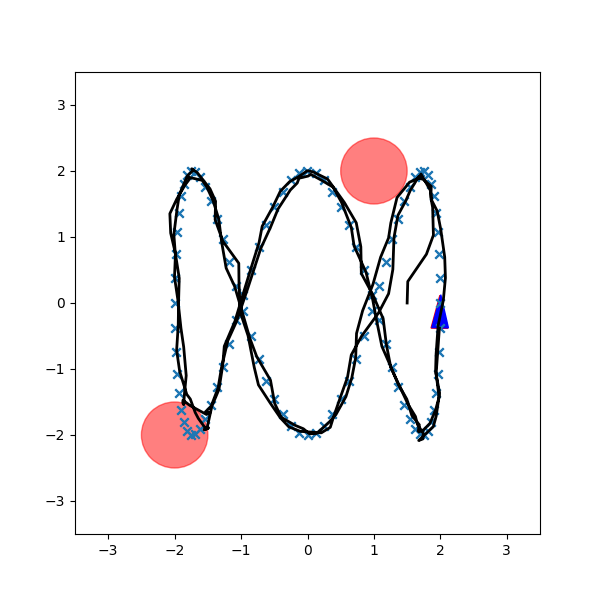
\includegraphics[width=\textwidth]{../fig/trajectory.cec.png}
        \caption{base line, $q=2, \gamma=0.9$}
        \label{fig:base}
        \end{subfigure}
    \hfill
    \begin{subfigure}[b]{0.3\textwidth}
        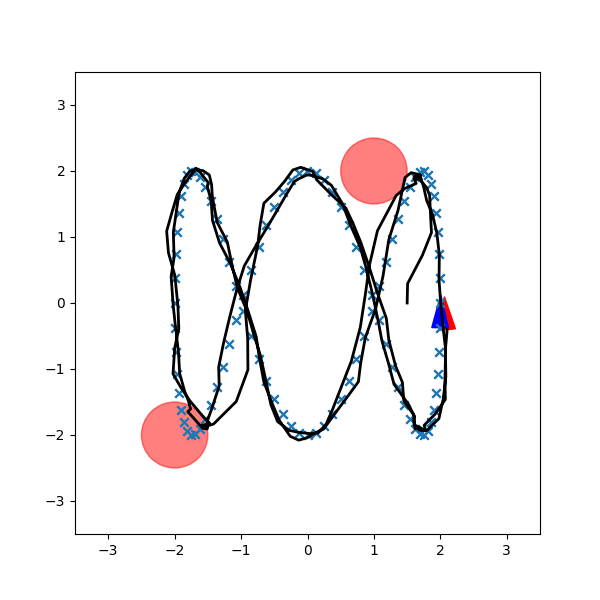
\includegraphics[width=\textwidth]{../fig/trajectory.cec.q_0.png}
        \caption{$q=0$}
        \label{fig:q0}
    \end{subfigure}
    \hfill
    \begin{subfigure}[b]{0.3\textwidth}
        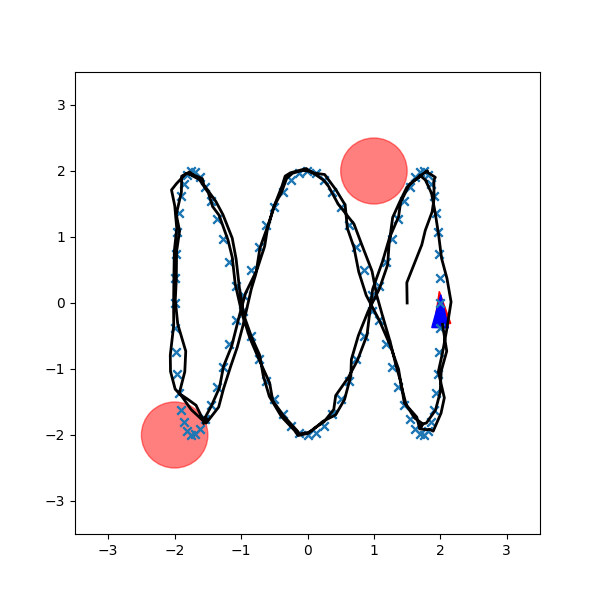
\includegraphics[width=\textwidth]{../fig/trajectory.cec.gamma_1.png}
        \caption{$\gamma=1$}
        \label{fig:gamma1}
    \end{subfigure}
    \caption{less important parameters}
    \label{fig:p}
\end{figure*}

\subsection{GPI}
Figure \ref{fig:gpi} shows the result of optimal policy extracted from Q-value iteration.
Compare to CEC results, it is clear that due to discretization granularity 
the GPI's control is less refined. However, the advantage of GPI is it online runtime.
Only one table lookup can decide the current control, which can be significant in 
latency sensitive and/or small time interval applications.
\end{document}
